% A skeleton file for producing Computer Engineering reports
% https://kgcoe-git.rit.edu/jgm6496/KGCOEReport_template

\documentclass[CMPE]{KGCOEReport}

% The following should be changed to represent your personal information
\newcommand{\classCode}{CMPE 160}  % 4 char code with number
\newcommand{\name}{Andrei Tumbar}
\newcommand{\LabSectionNum}{4}
\newcommand{\LabInstructor}{Mr.\ Byers}	% The slash is to tell LaTeX that the period is between words
												% not sentences so it spaces correctly. It won't appear in the
												% final pdf
\newcommand{\TAs}{Sam Myers \\ Kobe Balin \\ Georgi Thomas}
\newcommand{\LectureSectionNum}{1}
\newcommand{\LectureInstructor}{Mr.\ Cliver}
\newcommand{\exerciseNumber}{4}
\newcommand{\exerciseDescription}{Combinational Logic Circuit Design Using Boolean Algebra Simplification}
\newcommand{\dateDone}{February 6th}
\newcommand{\dateSubmitted}{February 13th}

\graphicspath{{./lab4_media/}}

\usepackage{circuitikz}
\usepackage{tikz}
\usepackage{multirow}
\usepackage{titlesec}
\usepackage{float}
\usepackage{pgfplots, pgfplotstable}
\usepackage{lmodern}
\usepackage{siunitx}

\usepackage{amsmath}

\DeclareFontFamily{U}{mathx}{\hyphenchar\font45}
\DeclareFontShape{U}{mathx}{m}{n}{ <-> mathx10 }{}
\DeclareSymbolFont{mathx}{U}{mathx}{m}{n}
\DeclareFontSubstitution{U}{mathx}{m}{n}
\DeclareMathAccent{\widebar}{\mathalpha}{mathx}{"73}

\makeatletter
\newcommand{\cwidebar}[2][0]{{\mathpalette\@cwidebar{{#1}{#2}}}}
\newcommand{\@cwidebar}[2]{\@cwideb@r{#1}#2}
\newcommand{\@cwideb@r}[3]{%
  \sbox\z@{$\m@th#1\mkern-#2mu#3\mkern#2mu$}%
  \widebar{\box\z@}%
}
\makeatother

\setcounter{secnumdepth}{2}

\def\coord(#1){coordinate(#1)}
\def\coord(#1){node[circle, red, draw, inner sep=1pt,pin={[red, overlay, inner sep=0.5pt, font=\tiny, pin distance=0.1cm, pin edge={red, overlay,}]45:#1}](#1){}}
\def\coordd(#1){node[circle, red, draw, inner sep=1pt,pin={[red, overlay, inner sep=0.5pt, font=\tiny, pin distance=0.1cm, pin edge={red, overlay,}]-45:#1}](#1){}}

\begin{document}
\maketitle

\section*{Abstract}
In this laboratory exercise, a circuit was implemented for a 3-input, 4-output function. The second (\(N_1\)) and third (\(N_2\)) inputs were representing a 2-bit binary number (N), the first input (\(C\)) was used as a control switch. When the control switch has a logical 0, the 4-bit out represented \(N^2\). When \(C\) is a logical 1, the output represents \(5N\). The min-terms were acquired from the 4-bit output (\(W\), \(X\), \(Y\), \(Z\)). The boolean expressions were then simplified. A circuit diagram was drawn to implement the function in Quartus II. Outputs were simulated in ModelSim using every possible input. The circuit was then built on a breadboard using ICs.

\section*{Design Methodology}

\subsection*{Truth Table}

A truth table was generated to denote the outputs from a set of inputs for the function.

\begin{table}[h]
\renewcommand{\arraystretch}{1.2}
\setlength{\tabcolsep}{12pt}
\caption{Truth Table for mathematical operations \(N^2\) and \(5N\)}
\begin{center}
\begin{tabular}{c|c|c|c||c|c|c|c|c}
\cline{2-8}
& C & \(N_1\) & \(N_0\) & W & X & Y & Z & \\\cline{2-8}
{\scriptsize 0} & 0 & 0 & 0 & 0 & 0 & 0 & 0 & \multirow{4}{*}{\(N^2\)}\\\cline{2-8}
{\scriptsize 1} & 0 & 0 & 1 & 0 & 0 & 0 & 1\\\cline{2-8}
{\scriptsize 2} & 0 & 1 & 0 & 0 & 1 & 0 & 0\\\cline{2-8}
{\scriptsize 3} & 0 & 1 & 1 & 1 & 0 & 0 & 1\\\cline{2-9}
{\scriptsize 4} & 1 & 0 & 0 & 0 & 0 & 0 & 0 & \multirow{4}{*}{\(5N\)}\\\cline{2-8}
{\scriptsize 5} & 1 & 0 & 1 & 0 & 1 & 0 & 1\\\cline{2-8}
{\scriptsize 6} & 1 & 1 & 0 & 1 & 0 & 1 & 0\\\cline{2-8}
{\scriptsize 7} & 1 & 1 & 1 & 1 & 1 & 1 & 1\\\cline{2-8}

\end{tabular}
\end{center}
\label{tab:TRUTH}
\end{table}

Table \ref{tab:TRUTH} shows the inputs and outputs of the function. When \(C\) is a 0, the 4-bit output \(WXYZ\), represents \(N^2\). When \(C\) is 1, the output is \(5N\). Each output column can be treated as their own function:

\begin{equation}
\label{eq:1}
W = \sum_{}^{}m(3,6,7)
\end{equation}

\begin{equation}
\label{eq:2}
X = \sum_{}^{}m(2,5,7)
\end{equation}
\begin{equation}
\label{eq:3}
Y = \sum_{}^{}m(6,7)
\end{equation}
\begin{equation}
\label{eq:4}
Z = \sum_{}^{}m(1,3,5,7)
\end{equation}

The min-terms above can be expanded to their boolean expressions in terms of \(C\), \(N_1\), and \(N_0\) and then simplified.

\begin{equation*}
W = \widebar{C}N_1N_0 + CN_1\widebar{N_0} + CN_1N_0
\end{equation*}
\begin{align*}
    &= \widebar{C}N_1N_0 + CN_1(\widebar{N_0} + N_0) && \text{Distributive property}\\
    &= \widebar{C}N_1N_0 + CN_1 && \text{Identity Law}\\
    &= N_1(\widebar{C}N_0 + C) && \text{Distributive property}\\
    &= N_1(N_0 + C) && \text{Consensus Theorem}
\end{align*}

Each term from the min-term in equation \ref{eq:1} was expressed by a sum of products. It was then simplified using the rules of boolean algrebra. The same technique was applied for \(X\), \(Y\), and \(Z\)

\begin{equation*}
X = \widebar{C}N_1\widebar{N_0} + C\widebar{N_1}N_0 + CN_1N_0
\end{equation*}
\begin{align*}
    &= \widebar{C}N_1\widebar{N_0} + CN_0(\widebar{N_1} + N_1) && \text{Distributive property}\\
    &= \widebar{C}N_1\widebar{N_0} + CN_0 && \text{Identity Law}\\
    &= (\widebar{C}\widebar{N_0})N_1 + CN_0 && \text{Associative Property}\\
    &= \widebar{(C + N_0)}N_1 + CN_0 && \text{De-Morgan's Law}
\end{align*}

The last step was done in order to reuse the output from the \(N_0 + C)\) OR gate in the \(W\) expression. This way a 3-input NAND would not need to be used.

\begin{equation*}
Y = CN_1\widebar{N_0} + CN_1N_0
\end{equation*}
\begin{align*}
    &= CN_1(\widebar{N_0} + N_0) && \text{Distributive property}\\
    &= CN_1 && \text{Identity Law}\\
\end{align*}

\begin{equation*}
Z = \widebar{C}\widebar{N_1}N_0 + \widebar{C}N_1N_0 + C\widebar{N_1}N_0 + CN_1N_0
\end{equation*}
\begin{align*}
    &= \widebar{C}\widebar{N_1}N_0 + \widebar{C}N_1N_0 + CN_0(\widebar{N_1} + N_1) && \text{Distributive property}\\
    &= \widebar{C}\widebar{N_1}N_0 + \widebar{C}N_1N_0 + CN_0 && \text{Identity Law}\\
    &= \widebar{C}N_0(\widebar{N_1} + N_1) + CN_0 && \text{Distributive property}\\
    &= \widebar{C}N_0 + CN_0 && \text{Identity Law}\\
    &= N_0(\widebar{C} + C) && \text{Distributive property}\\
    &= N_0 && \text{Identity Law}\\
\end{align*}

The simplification for \(Z\) initially looks like a mistake because of its simplicity. However, the coresponding rows where \(Z\) was a 1 were identical to the \(N_0\) column. In the case of \(Y\), no gates could be reused from the first two functions. \par

\pagebreak

A schematic diagram was drawn to implement these functions in one circuit. The circuit has three input pins and four output pins.

\begin{figure}[htbp]
	\centering
	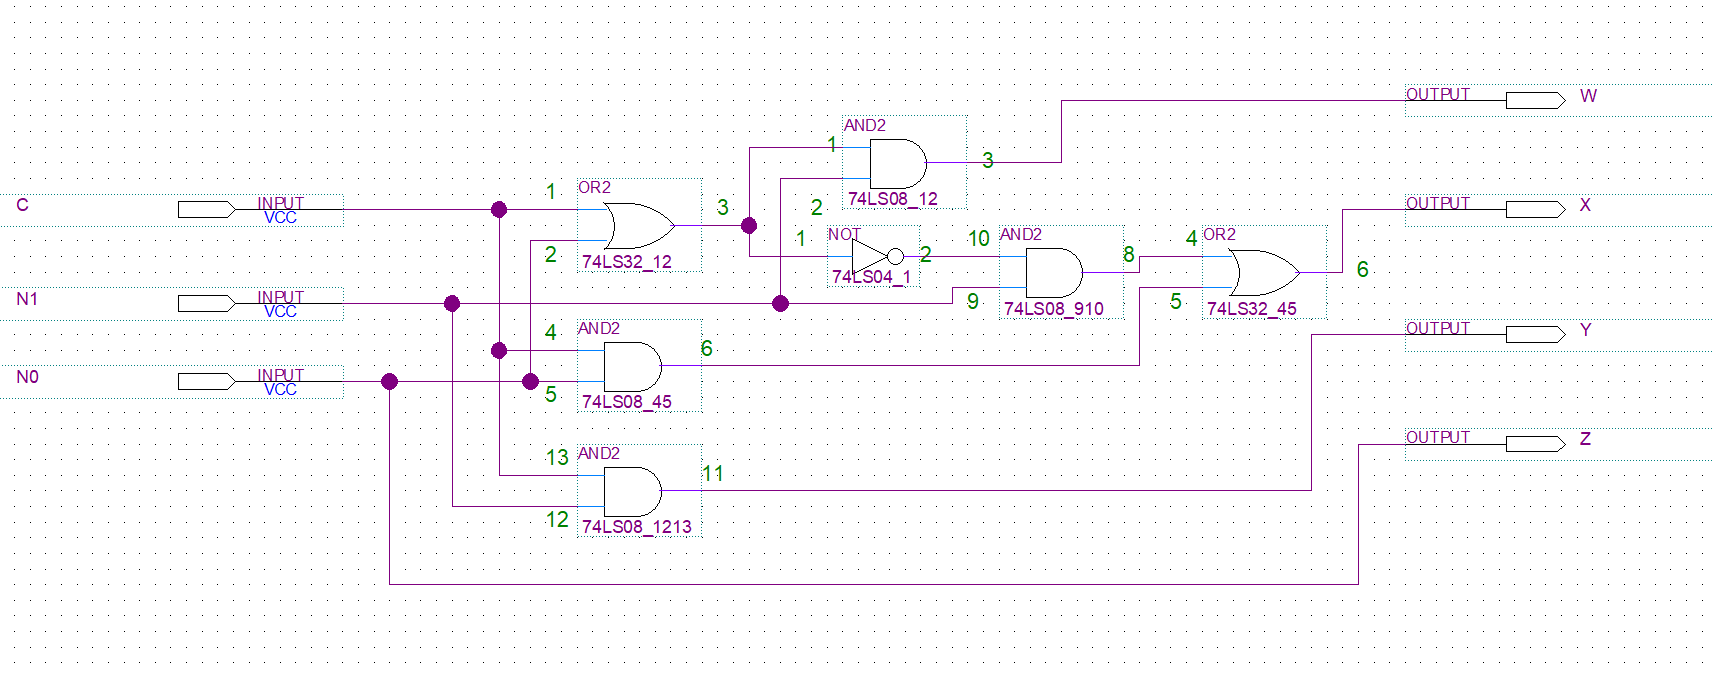
\includegraphics[width=\textwidth]{circuit}
	\caption{Circuit diagram for function with 3-inputs and 4-outputs.}
	\label{fig:cir}
\end{figure}

Figure \ref{fig:cir} was drawn in Quartus II using the circuit diagram function. Outputs \(Y\) and \(Z\) are easy to follow being one or zero gates. The first two outputs reused the OR gate labeled 74LS32\_12. Each gate was labeled according to its IC name followed by the input pins used. The green labels are the pin numbers for both output and input on the ICs.\par

The above circuit was run through a simulation in ModelSim to show the resultant outputs from all of the input combinations.

\begin{figure}[htbp]
	\centering
	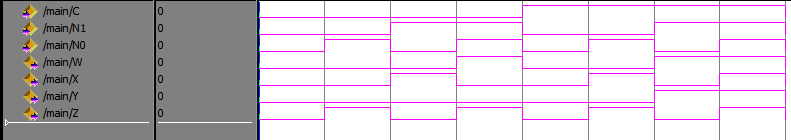
\includegraphics[width=\textwidth]{modelsim}
	\caption{Simulation of the circuit using ModelSim.}
	\label{fig:sim}
\end{figure}

Figure \ref{fig:sim}'s first three rows show the inputs. The final four show the output pins. The input and output combinations match those in Table \ref{tab:TRUTH}. This means that the circuit was set up correctly.

\section*{Results and Analysis}

THe hardware was contructed and tested using 3 chips. An AND, OR, and INVERT chip was needed to implement the circuit shown in Figure \ref{fig:cir}. The DC power supply was configured to produce a $5\,\si\volt$ source and a maximum of $0.1\,\si\ampere$. The first three switch were configured as inputs and four of the LED were wired as outputs. All of the input combinations of the input switches matched the output combinations on the LEDs as in Table \ref{tab:TRUTH}.

\section*{Conclusion}

This exercise implemented a 3-input, 4-output function, F, first using boolean algebra and then translated to a circuit. The circuit was tested in ModelSim to verify the correct combination of gates were used. Finally the circuit was implemented on a breadboard and was tested using the input switches and the LEDs as output. The purpose of this exercise was to design a circuit completely from the definition to the hardware implementation.

\section*{Questions}

\begin{enumerate}
  \item A total of 6 two-input gates were used in this circuit design. This was made possible by using DeMorgan's Law to further simplify $X$ and therefore use one of the gate outputs of $W$. A total of four 2-input AND gates and two 2-input OR gates were used.

  \item A total of 3 ICs were used. Every 2-input, 1 output IC holds four gates. Because the OR and AND gate counts did not exceed 4, one chip could be used for each. In the case of the inverter, a 1-input, 1-output gate, a total of 6 inverter gates are inside the chip. Only one inverter was needed in order to implement the circuit. Therefore, 1x 74LS08 2-input AND gate, 1x 74LS32 2-input OR gate, and 1x 74LS04 1-input inverter chips were used.
\end{enumerate}

\end{document}
